% abtex2-modelo-artigo.tex, v-1.9.2 laurocesar
% Copyright 2012-2014 by abnTeX2 group at http://abntex2.googlecode.com/ 
%

% ------------------------------------------------------------------------
% ------------------------------------------------------------------------
% abnTeX2: Modelo de Artigo Acadêmico em conformidade com
% ABNT NBR 6022:2003: Informação e documentação - Artigo em publicação 
% periódica científica impressa - Apresentação
% ------------------------------------------------------------------------
% ------------------------------------------------------------------------

\documentclass[
	% -- opções da classe memoir --
	article,			% indica que é um artigo acadêmico
	11pt,				% tamanho da fonte
	oneside,			% para impressão apenas no verso. Oposto a twoside
	a4paper,			% tamanho do papel. 
	% -- opções da classe abntex2 --
	%chapter=TITLE,		% títulos de capítulos convertidos em letras maiúsculas
	%section=TITLE,		% títulos de seções convertidos em letras maiúsculas
	%subsection=TITLE,	% títulos de subseções convertidos em letras maiúsculas
	%subsubsection=TITLE % títulos de subsubseções convertidos em letras maiúsculas
	% -- opções do pacote babel --
	english,			% idioma adicional para hifenização
	brazil,				% o último idioma é o principal do documento
	sumario=tradicional
	]{abntex2}


% ---
% PACOTES
% ---

% ---
% Pacotes fundamentais 
% ---
\usepackage{lmodern}			% Usa a fonte Latin Modern
\usepackage[T1]{fontenc}		% Selecao de codigos de fonte.
\usepackage[utf8]{inputenc}		% Codificacao do documento (conversão automática dos acentos)
\usepackage{indentfirst}		% Indenta o primeiro parágrafo de cada seção.
\usepackage{nomencl} 			% Lista de simbolos
\usepackage{color}				% Controle das cores
\usepackage{graphicx}			% Inclusão de gráficos
\usepackage{microtype} 			% para melhorias de justificação

\usepackage{cmap}				% Mapear caracteres especiais no PDF
% ---
% ---
		
\usepackage{amsmath}
% ---
% Pacotes adicionais, usados apenas no âmbito do Modelo Canônico do abnteX2
% ---
\usepackage{lipsum}				% para geração de dummy text
% ---
		
% ---
% Pacotes de citações
% ---
\usepackage[brazilian,hyperpageref]{backref}	 % Paginas com as citações na bibl
\usepackage[alf]{abntex2cite}	% Citações padrão ABNT
% ---

% ---
% Configurações do pacote backref
% Usado sem a opção hyperpageref de backref
\renewcommand{\backrefpagesname}{Citado na(s) página(s):~}
% Texto padrão antes do número das páginas
\renewcommand{\backref}{}
% Define os textos da citação
\renewcommand*{\backrefalt}[4]{
	\ifcase #1 %
		Nenhuma citação no texto.%
	\or
		Citado na página #2.%
	\else
		Citado #1 vezes nas páginas #2.%
	\fi}%
% ---

% ---
% Informações de dados para CAPA e FOLHA DE ROSTO
% ---
\titulo{Modelo Canônico de\\ Artigo científico com \abnTeX}
\autor{Equipe \abnTeX\thanks{\url{http://abntex2.googlecode.com/}} \and Lauro
César
Araujo\thanks{laurocesar@laurocesar.com}}
\local{Brasil}
\data{2014, v-1.9.2}
% ---

% ---
% Configurações de aparência do PDF final

% alterando o aspecto da cor azul
\definecolor{blue}{RGB}{41,5,195}

% informações do PDF
\makeatletter
\hypersetup{
     	%pagebackref=true,
		pdftitle={\@title}, 
		pdfauthor={\@author},
    	pdfsubject={Modelo de artigo científico com abnTeX2},
	    pdfcreator={LaTeX with abnTeX2},
		pdfkeywords={abnt}{latex}{abntex}{abntex2}{atigo científico}, 
		colorlinks=true,       		% false: boxed links; true: colored links
    	linkcolor=blue,          	% color of internal links
    	citecolor=blue,        		% color of links to bibliography
    	filecolor=magenta,      		% color of file links
		urlcolor=blue,
		bookmarksdepth=4
}
\makeatother
% --- 

% ---
% compila o indice
% ---
\makeindex
% ---

% ---
% Altera as margens padrões
% ---
\setlrmarginsandblock{3cm}{3cm}{*}
\setulmarginsandblock{3cm}{3cm}{*}
\checkandfixthelayout
% ---

% --- 
% Espaçamentos entre linhas e parágrafos 
% --- 

% O tamanho do parágrafo é dado por:
\setlength{\parindent}{1.3cm}

% Controle do espaçamento entre um parágrafo e outro:
\setlength{\parskip}{0.2cm}  % tente também \onelineskip

% Espaçamento simples
\SingleSpacing

% ----
% Início do documento
% ----
\begin{document}

% Retira espaço extra obsoleto entre as frases.
\frenchspacing 

% ----------------------------------------------------------
% ELEMENTOS PRÉ-TEXTUAIS
% ----------------------------------------------------------

%---
%
% Se desejar escrever o artigo em duas colunas, descomente a linha abaixo
% e a linha com o texto ``FIM DE ARTIGO EM DUAS COLUNAS''.
%\twocolumn[    		% INICIO DE ARTIGO EM DUAS COLUNAS
%
%---
% página de titulo
\maketitle

% resumo em português
\begin{resumoumacoluna}
 Conforme a ABNT NBR 6022:2003, o resumo é elemento obrigatório, constituído de
 uma sequência de frases concisas e objetivas e não de uma simples enumeração
 de tópicos, não ultrapassando 250 palavras, seguido, logo abaixo, das palavras
 representativas do conteúdo do trabalho, isto é, palavras-chave e/ou
 descritores, conforme a NBR 6028. (\ldots) As palavras-chave devem figurar logo
 abaixo do resumo, antecedidas da expressão Palavras-chave:, separadas entre si por
 ponto e finalizadas também por ponto.
 
 \vspace{\onelineskip}
 
 \noindent
 \textbf{Palavras-chaves}: latex. abntex. editoração de texto.
\end{resumoumacoluna}

% ]  				% FIM DE ARTIGO EM DUAS COLUNAS
% ---

% ----------------------------------------------------------
% ELEMENTOS TEXTUAIS
% ----------------------------------------------------------
\textual

% ----------------------------------------------------------
% Introdução
% ----------------------------------------------------------
\newpage
\section*{Introdução}
\addcontentsline{toc}{section}{Introdução}

Este documento e seu código-fonte são exemplos de referência de uso da classe
%\textsf - Usado para produzir material em modo texto em fonte sans serif
\textsf{abntex2} e do pacote \textsf{abntex2cite}. O documento exemplifica a 
elaboração de publicação periódica científica impressa produzida conforme a ABNT
%\emph - Usado para produzir material em modo texto italico 
NBR 6022:2003 \emph{Informação e documentação - Artigo em publicação periódica
científica impressa - Apresentação}.

A expressão ``Modelo canônico'' é utilizada para indicar que \abnTeX\ não é
modelo específico de nenhuma universidade ou instituição, mas que implementa tão
somente os requisitos das normas da ABNT. Uma lista completa das normas
%para citar uma parte do texto // para texStudio usa "\cite{livro1}"
% e para imagens \ref{figura1} ,\ref{equacao1}
%onde por exemplo a imagem teria o label como figura1
%\begin{figure}[!htb] 
%	\label{figura1} 
%	\includegraphics[width = 190pt, height = 160pt]{simpson1.png} 
%\end{figure}
observadas pelo \abnTeX\ é apresentada em \citeonline{abntex2classe}.

Sinta-se convidado a participar do projeto \abnTeX! Acesse o site do projeto em
%colocar a url em destaque
\url{http://abntex2.googlecode.com/}. Também fique livre para conhecer,
estudar, alterar e redistribuir o trabalho do \abnTeX, desde que os arquivos
modificados tenham seus nomes alterados e que os créditos sejam dados aos
autores originais, nos termos da ``The \LaTeX\ Project Public
License
%para colocar esse link no 'rodape'
%''\footnote{\url{http://www.latex-project.org/lppl.txt}}.


Encorajamos que sejam realizadas customizações específicas deste documento.
Porém, recomendamos que ao invés de se alterar diretamente os arquivos do
\abnTeX, distribua-se arquivos com as respectivas customizações. Isso permite
que futuras versões do \abnTeX~não se tornem automaticamente incompatíveis com
as customizações promovidas. Consulte \citeonline{abntex2-wiki-como-customizar}
par mais informações.

Este exemplo deve ser utilizado como complemento do manual da classe
\textsf{abntex2} \cite{abntex2classe}, dos manuais do pacote
\textsf{abntex2cite} \cite{abntex2cite,abntex2cite-alf} e do manual da classe
\textsf{memoir} \cite{memoir}. Consulte o \citeonline{abntex2modelo} para obter
exemplos e informações adicionais de uso de \abnTeX\ e de \LaTeX.



\newpage
\chapter{Figuras}
imagens
\begin{figure} [hbt] 
%% hbt SIGNIFICA QUE ELE PRIMEIRO VAI TENTAR COLOCAR A IMAGEM NESTE LUGAR (h de "here"). SENÃO DER, ELE TENTA COLOCAR MAIS PRA BAIXO (b de "bottom"). SENÃO ELE COLOCA MAIS PARA CIMA (t de "top").
\centering
\label{Rotulo}
\label{figura1} 
\caption{Exemplo de interpolação inadequada}
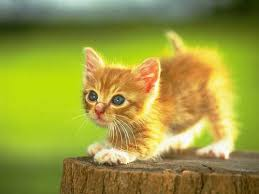
\includegraphics[width=0.55\textwidth]{gato.jpg}
\end{figure}

\begin{figure} [hbt] 
%% hbt SIGNIFICA QUE ELE PRIMEIRO VAI TENTAR COLOCAR A IMAGEM NESTE LUGAR (h de "here"). SENÃO DER, ELE TENTA COLOCAR MAIS PRA BAIXO (b de "bottom"). SENÃO ELE COLOCA MAIS PARA CIMA (t de "top").
\centering
\label{Rotulo}
\label{figura2} 
\caption{Exemplo de interpolação inadequada}
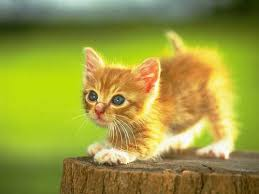
\includegraphics[width=0.55\textwidth]{gato.jpg}
\end{figure}

\newpage

















\newpage
% ----------------------------------------------------------
% Seção de explicações
% ----------------------------------------------------------
\section{Exemplos de comandos e expressões matemáticas}

\subsection{Margens}

As imagens no latex, pode ser adicionada de maneira simples

\subsection{Duas colunas}

É comum que artigos científicos sejam escritos em duas colunas. Para isso,
adicione a opção \texttt{twocolumn} à classe do documento, como no exemplo:

\begin{verbatim}
   \documentclass[article,11pt,oneside,a4paper,twocolumn]{abntex2}
\end{verbatim}

É possível com o latex exvcrever de maneira simples variaveis equações
como por exemplo, os seguintes exemplos
a opção \texttt{label} devem ser escrita se caso precise citar ela em outro local do texto

\begin{equation} \label{equacaosimpson2}
I = H/3 \times [f(X_1) + 4 \times f(X_2) + f(X_3)]
\end{equation} 


\subsection{Somatorio simples no latex e permitir \texttt{citacao}}

O latex mantem as expressões bem definidas, não é atoa que o latex é muito bem
visto quando usado na area academica de exatas, por manter a construções de perfeitas
equações nas quais mantem um aspecto invejavel:

\begin{equation} \label{equacaosimpsons1}
S1 = \sum_{i = 1,3,5..}^{N-1} f(x_i)
\end{equation} 


Quando um documento é produzido com a opção \texttt{twocolumn}, a classe
\textsf{abntex2} automaticamente altera o recuo padrão de 4 cm, definido pela
ABNT NBR 10520:2002 seção 5.3, para 1.8 cm.

%PARTE MATEMATICA, COLOCANDO EQUAÇÕES MATRIZES NO LATEX
\section{Matematica no latex}

Diferentes estilos de cabeçalhos e rodapés podem ser criados usando os
recursos padrões do \textsf{memoir}.
Para referenciar uma equação faça \ref{integralexemplo}, logo tera um 'link'
para a equação

Um estilo próprio de cabeçalhos e rodapés pode ser diferente para páginas pares
e ímpares. Observe que a diferenciação entre páginas pares e ímpares só é
utilizada se a opção \texttt{twoside} da classe \textsf{abntex2} for utilizado.
Caso contrário, apenas o cabeçalho padrão da página par (\emph{even}) é usado.

Veja o exemplo abaixo cria um estilo chamado \texttt{meuestilo}. O código deve
ser inserido no preâmbulo do documento. na equação abaixo temos um exemplo de integral.



\begin{equation} \label{integralexemplo}
\int_{0}^{2}x\epsilon ^(-3x^2) dx
\end{equation} 

%tabela
%$$\begin{tabular}{|c|c|c|c|c|}\hline
%{.} & A  & B  & C  \\\hline
%1   & A1 & B1 & C1 \\\hline
%2   & A2 & B2 & C2 \\\hline
%\end{tabular}$$

No exemplo abaixo temos um exemplo de uma toma de varios elementos, no qual estão todos organizados. Percebemos a 
facilidade que o latex nos trás.

\begin{eqnarray*}
\theta &=& a+b+c+d+e+f+ \\
& & g+h+i+j+k+l+m+n+ \\
& & o+p+q+r+s+t+u+v+w+x+y+z+1+2+3
\end{eqnarray*}

Abaixo, vemos como são monstadas matrizes no latex, de forma simples e prática, no latex você monta matrizes sem
qualquer trabalho.
$$
\begin{matrix}
a & b \\
c & d
\end{matrix}
\quad
\begin{pmatrix}
a & b \\
c & d
\end{pmatrix}
$$
$$
\begin{bmatrix}
a & b \\
c & d
\end{bmatrix}
\quad
\begin{vmatrix}
a & b \\
c & d
\end{vmatrix}
\quad
\begin{Vmatrix}
a & b \\
c & d
\end{Vmatrix}
$$

O latex, trabalha muito bem com funções, que nas mesmas podem aparecer o uso de cochetes, onde são adicionados nas equações
de maneira pratica e simples 

\begin{equation}
f(n) = \left \{ \begin{matrix} n/2, & \mbox{se }n\mbox{ é par} \\ 3n+1, & \mbox{se }n\mbox{ é ímpar} \end{matrix} \right.
\end{equation}

%EQUAÇÕES NO MEIO DO TEXTO
uando a equação possui mais do que uma incógnita, podemos expressar o grau em relação à equação como um todo. Para isso, devemos avaliar o grau de cada monômio da equação. \(x^2 + y^2 = z^2\)  Observe o exemplo: Dada a equação: \[ x^n + y^n = z^n \] identifique o seu grau em relação à incógnita x e y. Em seguida, encontre o seu grau geral.


   
Outras informações sobre cabeçalhos e rodapés estão disponíveis na seção 7.3 do
%essa citação esta no arquivo separado com os demais dados do autor citado
manual do \textsf{memoir} \cite{memoir}.

\section{Exemplos de citações e referências }

Este modelo de artigo é limitado em número de exemplos de comandos, pois são
apresentados exclusivamente comandos diretamente relacionados com a produção de
artigos.

Para exemplos adicionais de \abnTeX\ e \LaTeX, como inclusão de figuras,
fórmulas matemáticas, citações, e outros, consulte o documento \citeonline{abntex2modelo}.

\section{Consulte o manual da classe \textsf{abntex2}}

Consulte o manual da classe \textsf{abntex2} \cite{abntex2classe} para uma
referência completa das macros e ambientes disponíveis.

% ---
% Finaliza a parte no bookmark do PDF, para que se inicie o bookmark na raiz
% ---
\bookmarksetup{startatroot}% 
% ---------------------------------------------------------------------------
\newpage
% ---
% Conclusão
% ---
\section*{Considerações finais}
\addcontentsline{toc}{section}{Considerações finais}

\lipsum[1] % insere testo aleatorio

\begin{citacao}
\lipsum[2] %insere testo aleatorio
\end{citacao}

\lipsum[3] %insere testo aleatorio

% ----------------------------------------------------------
% ELEMENTOS PÓS-TEXTUAIS
% ----------------------------------------------------------
\postextual

% ---
% Título e resumo em língua estrangeira
% ---

% \twocolumn[    		% INICIO DE ARTIGO EM DUAS COLUNAS

% titulo em inglês


% ]  				% FIM DE ARTIGO EM DUAS COLUNAS
% ---

% ----------------------------------------------------------
% Referências bibliográficas
% ----------------------------------------------------------
\newpage
\bibliography{abntex2-modelo-references}

% ----------------------------------------------------------
% Glossário
% ----------------------------------------------------------
%
% Há diversas soluções prontas para glossário em LaTeX. 
% Consulte o manual do abnTeX2 para obter sugestões.
%
%\glossary

% ----------------------------------------------------------
% Apêndices
% ----------------------------------------------------------
\newpage
% ---
% Inicia os apêndices
% ---
\begin{apendicesenv}

% ----------------------------------------------------------
\chapter{Nullam elementum urna vel imperdiet sodales elit ipsum pharetra ligula
ac pretium ante justo a nulla curabitur tristique arcu eu metus}
% ----------------------------------------------------------
\lipsum[55-57]

\end{apendicesenv}
% ---

% ----------------------------------------------------------
% Anexos
% ----------------------------------------------------------
\cftinserthook{toc}{AAA}
% ---
% Inicia os anexos
% ---
%\anexos
\newpage
\begin{anexosenv}

% ---
\chapter{Cras non urna sed feugiat cum sociis natoque penatibus et magnis dis
parturient montes nascetur ridiculus mus}
% ---

\lipsum[31]

\end{anexosenv}

\end{document}
